\begin{tikzpicture}
  \colorlet{cavl}{color3}
  \colorlet{cvio}{color5}
  \colorlet{csensor}{color2}
  \colorlet{cactuator}{color2}
  \colorlet{cos}{white}
  \colorlet{chw}{white}
  
  \tikzstyle{sensor}=[fill=csensor]
  \tikzstyle{actuator}=[fill=cactuator]
  \tikzstyle{os}=[fill=cos]
  \tikzstyle{avl}=[fill=cavl]
  \tikzstyle{vio}=[fill=cvio]
  \tikzstyle{eventtext}=[font=\small\ttfamily]
  \tikzstyle{event}=[->, thick, eventtext]
  \tikzstyle{evio}=[event, draw=cvio]
  \tikzstyle{eavl}=[event, draw=cavl]
  \tikzstyle{trustedhw}=[fill=chw]
  \tikzstyle{device}=[draw, thin, rounded corners, trustedhw]
  
  \newcommand{\swmodule}[3]{\node[#2] (#1) {#3}; \\}
  \newcommand{\hwnode}[4]{
    \matrix[matrix of nodes,
            draw, trustedhw,
            minimum height=80, minimum width=83,
            ampersand replacement=\&,
            nodes={draw, text width=2cm, align=center,
                   minimum height=0, minimum width=0}, #2] (#1) {
      #4
      \swmodule{}{os}{Untrusted OS}
    };
    \node[yshift=-10pt] at (#1.south) {#3};
  }
  \newcommand{\hwnodesmall}[4]{
    \matrix[matrix of nodes,
            draw, trustedhw,
            minimum height=48, minimum width=83,
            ampersand replacement=\&,
            nodes={draw, text width=2cm, align=center,
                   minimum height=0, minimum width=0}, #2] (#1) {
      #4
      \swmodule{}{os}{Untrusted OS}
    };
    \node[yshift=-10pt] at (#1.south) {#3};
  }
   
  \newcommand{\sensor}[2]{
    \draw[white] (#1) -- ++(up:20pt) coordinate (Start)
%                      -- ++(right:10pt)
                         ++(up:20pt) coordinate (Top)
%                      -- ++(10pt, -5pt)
                      -- ++(right:30pt) coordinate (End);
    \draw[thick] (#1) -- ++(up:20pt);
    \node[inner sep=0pt] at ([xshift=15pt, yshift=27pt]#1) {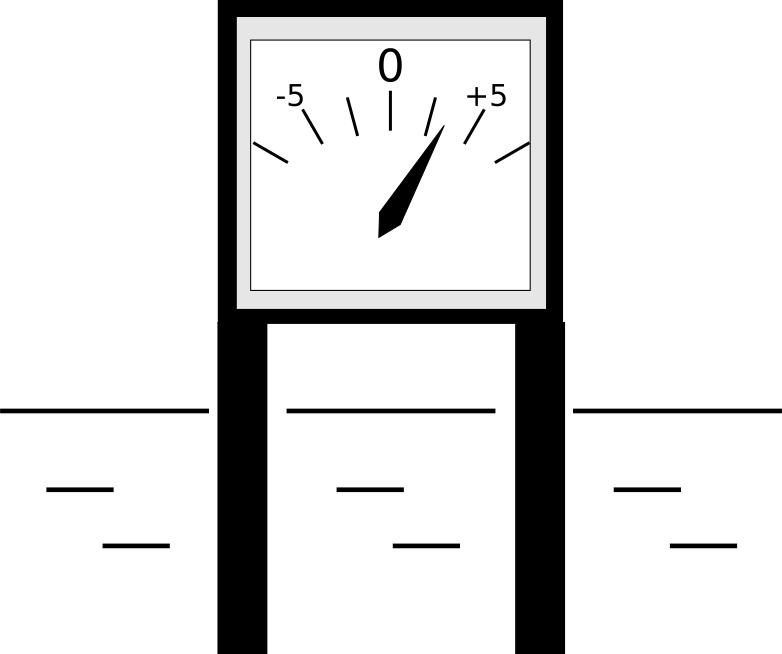
\includegraphics[width=0.08\textwidth]{graphics/clipart/moisture-meter.pdf}};
    \begin{pgfonlayer}{background}
      \node[device, fit={([yshift=-5pt]Start) (Top) (End)}, label=right:#2] {};
    \end{pgfonlayer}
  }
  
  \newcommand{\clock}[2]{
    \draw[thick] (#1) -- ++(left:15pt) coordinate (Start)
      foreach \i in {1,...,3} {
        -- ++(up:7pt) -- ++(left:5pt) -- ++(down:7pt) -- ++(left:5pt)
      } coordinate (End);
    \begin{pgfonlayer}{background}
      \node[device, fit={([yshift=-5pt]Start) ([yshift=12pt]End)}, label=#2] {};
    \end{pgfonlayer}
  }
  
  \newcommand{\display}[3]{
    \draw[thick] (#1) -- ++(right:15pt)
      node[device, anchor=west, label=#2,
           text width=50pt, align=center] (Disp-#1) {#3};
  }

  \hwnode{NP1}{}{$N_{S1}$}{
    \swmodule{SD1}{sensor}{Sensor driver}
    \swmodule{CD1}{sensor}{Clock driver}
    \swmodule{VioP1}{vio}{\module{FloS1}}
    \swmodule{AvlP1}{avl}{\module{AggS1}}
  }
  
  \sensor{SD1.165}{\dev{S1}}
  \clock{CD1.west}{\dev{T1}}
  
  \hwnode{NP2}{right=2 of NP1}{$N_{S2}$}{
    \swmodule{SD2}{sensor}{Sensor driver}
    \swmodule{CD2}{sensor}{Clock driver}
    \swmodule{VioP2}{vio}{\module{FloS2}}
    \swmodule{AvlP2}{avl}{\module{AggS2}}
  }
  
  \sensor{SD2.165}{\dev{S2}}
  \clock{CD2.west}{\dev{T2}}
  
  \hwnodesmall{NAGG}{below=of NP2}{$N_{\scriptsize\textit{Agg}}$}{
    \swmodule{Agg}{avl}{\module{Agg}}
  }
  
  \hwnode{ND1}{right=2 of NP2}{$N_{A}$}{
    \swmodule{DD1}{actuator}{Actuator driver}
    \swmodule{VioD}{vio}{\module{FloA}}
  }
  
%  \display{DD1.east}{\dev{D1}}{Violations: \\ None}
  \display{DD1.east}{\dev{A}}{Tap on/off \\
    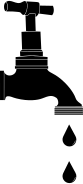
\includegraphics[width=0.25\textwidth]{graphics/clipart/tap-drops.pdf}}
  
  \hwnodesmall{ND2}{below=of ND1}{$N_{D}$}{
    \swmodule{DD2}{actuator}{Display driver}
    \swmodule{AvlD}{avl}{\module{AggD}}
  }
  
  \display{DD2.east}{\dev{D}}{Moisture: \\ 55\%}
  
  \draw[evio] (CD1.185)   -- ++(left:4pt)  |- (VioP1.west) coordinate[pos=.25] (LabelT1);
  \draw[evio] (SD1.east)  -- ++(right:6pt) |- (VioP1.5) coordinate[pos=.25] (LabelB1);
  \draw[evio] (CD2.185)   -- ++(left:4pt)  |- (VioP2.west) coordinate[pos=.25] (LabelT2);
  \draw[evio] (SD2.east)  -- ++(right:6pt) |- (VioP2.5) coordinate[pos=.25] (LabelB2);
  \draw[evio] (VioD.east) -- ++(right:6pt) |- (DD1.350) coordinate[pos=.25] (LabelD);
  
  \draw[evio, rounded corners=20pt]
      (VioP1.355)
      -- ++(right:13pt)
      -- ++(20pt, 70pt)
      to[bend left] node[above]{Flooded} ++(right:130pt)
      -- ++(20pt, -50pt)
      --   (VioD.175);
  \draw[evio] (VioP2.355) to[bend right=10] node[below] {Flooded} (VioD.185);
  
  \draw[eavl] (SD1.west)  -- ++(left:6pt) |- (AvlP1.west);
  \draw[eavl] (SD2.west)  -- ++(left:6pt) |- (AvlP2.175);
  \draw[eavl] (AvlD.east) -- ++(right:6pt) |- (DD2.350) coordinate[pos=.25] (LabelD2);

  \draw[eavl] (AvlP1.east) to[out=0,   in=180]                coordinate (LabelM1) (Agg.185);
  \draw[eavl] (AvlP2.185)  to[out=180, in=180, looseness=0.7] coordinate (LabelM2) (Agg.175);
  \draw[eavl] (Agg.east)   to[bend right=10]                  node[below,
eventtext] {MoistChanged} (AvlD.west);

  \begin{scope}[inner sep=0, eventtext]
    \draw (LabelD)  to[bend left]  ++(10pt, -10pt)
                                   node[below right] {Tap};
    \draw (LabelD2)  to[bend left]  ++(10pt, -10pt)
                                   node[below right] {Display};
    \draw (LabelB1) to[bend left]  ++(10pt, 10pt)
                                   node[below right, rotate=90] {Sensor};
    \draw (LabelB2) to[bend left]  ++(10pt, 10pt)
                                   node[below right, rotate=90,
xshift=-25pt] {Sensor};
    \draw (LabelT1) to[bend right] ++(-10pt, -10pt)
                                   node[below left] {Tick};
    \draw (LabelT2) to[bend right] ++(-10pt, -10pt)
                                   node[below left] {Tick};
    \draw (LabelM2) to[bend right] ++(-8pt, 8pt)
                                   node[above, rotate=90] (CarMoved) {Moisture};
    \draw (LabelM1) to[bend left] (CarMoved.north);
  \end{scope}
\end{tikzpicture}
